%% Richard Wen
%% rwen@ryerson.ca


% *** INTRODUCTION ***


\section{Introduction} \label{introduction}

\IEEEPARstart{M}{achine} learning\footnote{Machine learning is a field of computer science that studies the computer's ability to automatically learn without being specifically programmed \cite{Samuel:2000}.} models have been used in important real-world applications such as identifying online criminal activity, forecasting stock markets, and diagnosing sicknesses \cite{Buczak:2016,Heaton:2017,Muandet:2017}. Recent machine learning research has led to advances in data security, financial trading, and medical diagnoses \cite{Deng:2014,deBruijne:2016}. Machine learning algorithms provide a set of instructions that enable computers to learn patterns in data without being specifically programmed \cite{LeCun:2015}. These patterns are used to produce models\footnote{A model refers to a representation of the data learned using an algorithm.} of the data where accuracies\footnote{Accuracy percentages measure the number of correctly predicted cases by the machine learning model in a given set of testing data, where values range from 0\% (no cases predicted correctly) to 100\% (all cases predicted correctly).} greater than 99\% are possible \cite{Schmidhuber:2015}.  These models often come with tunable values called \textit{hyperparameters} that affect the learning performance of the underlying algorithm. Hyperparameters can be tuned to produce models that achieve high accuracy in tasks such as speech recognition and visual object detection \cite{Deng:2013,Guo:2016,Bergstra:2011}. Instead of inventing algorithms or sophisticated methods, the hyperparameters in machine learning algorithms are often tuned to significantly improve model performance.

One of the disadvantages of hyperparameter tuning is that it requires user expertise in the algorithms and data used to produce the machine learning model. The simplest approach is to manual explore a set of hyperparameters. This approach, however, can subjectively differ from user to user such that the resulting machine learning model becomes difficult to reproduce and scientifically justify. Machine learning models also have the disadvantage of being time-consuming to produce, and only a small range of hyperparameter choices should be for the sake of feasibility. In the same amount of time, optimization methods can automatically discover better hyperparameters than manual exploration. Hyperparameter optimization methods can be used to automatically select optimal hyperparameters from predefined search and time constraints. These methods are easier to theoretically justify and reproduce to verify and improve upon research studies and machine learning models. Hyperparameter optimization methods automate the hyperparameter selection process to reduce selection bias, and the need for expertise in particular algorithms. This allows a variety of users with different backgrounds and knowledge to apply machine learning to real-world problems. This review investigated five papers, selected using journal quality measures and digital libraries, to provide a brief summary and discussion related to hyperparameter optimization methods for machine learning algorithms.

The goal of this review was to provide general knowledge and possible research directions of recent hyperparameter optimization methods for machine learning algorithms. A brief overview and evaluation of five selected papers from the past two years were provided. The review was done by selecting relevant and recent papers using digital library search queries and manual selection criteria. The selected papers were then summarized in terms of hyperparameter optimization methods, and experimental results. A discussion of the limitations, proposed improvements, and future directions evaluated and addressed the implications of the selected papers.

The remaining sections were organized as follows:

\begin{itemize}
  \item \textbf{Section \ref{methods}} detailed the methods used for digital library selection, paper selection, and reviewing selected papers
  \item \textbf{Section \ref{results}} presented the results of the paper selection process detailed in Section \ref{methods} and summarizes the selected papers
  \item \textbf{Section \ref{discussion}} discussed the limitations, proposed improvements, and future directions relative to the selected papers from Section \ref{results}
  \item \textbf{Section \ref{conclusion}} provided concluding remarks and implications
\end{itemize}


% *** METHODS***


\section{Methods} \label{methods}
This section explains the paper selection requirements and process. Reputable digital libraries with search engines were identified by exploring journal citation reports in Section\ref{digital-library-selections}. Automatic search queries from the identified digital libraries were then used to filter for potential papers in Section \ref{automatic-search-queries}. Section \ref{manual-selection-criteria} details the manual selection criteria used to filter these potential papers for the selected papers in this review. The review procedure in Section \ref{review-procedure} consisted of identifying and summarizing methods and models from the selected papers for a discussion of method and model limitations, improvements, and future directions.


\subsection{Digital Library Selections} \label{digital-library-selections}

The papers selected for this review were found using the search engines available in the Association for Computing Machinery (ACM) and Institute of Electrical and Electronics Engineers (IEEE) Xplore digital libraries \cite{ACM:2017,IEEE:2017}. A search for the top journals in computer science by journal impact factor \cite{Garfield:2006b} was done using the InCites journal citation reports web tool \cite{Clarivate:2017a} (See Appendix \ref{appendix:incites_search}). A majority of ACM and IEEE journals were found to be in the first quartile of journal impact factor values for the computer science category. A visualization of the top 25 journals in computer science by journal impact factor in 2016 is shown in Figure \ref{figure:cs_jif_graph}.

\begin{figure}[!t]
	\centering
	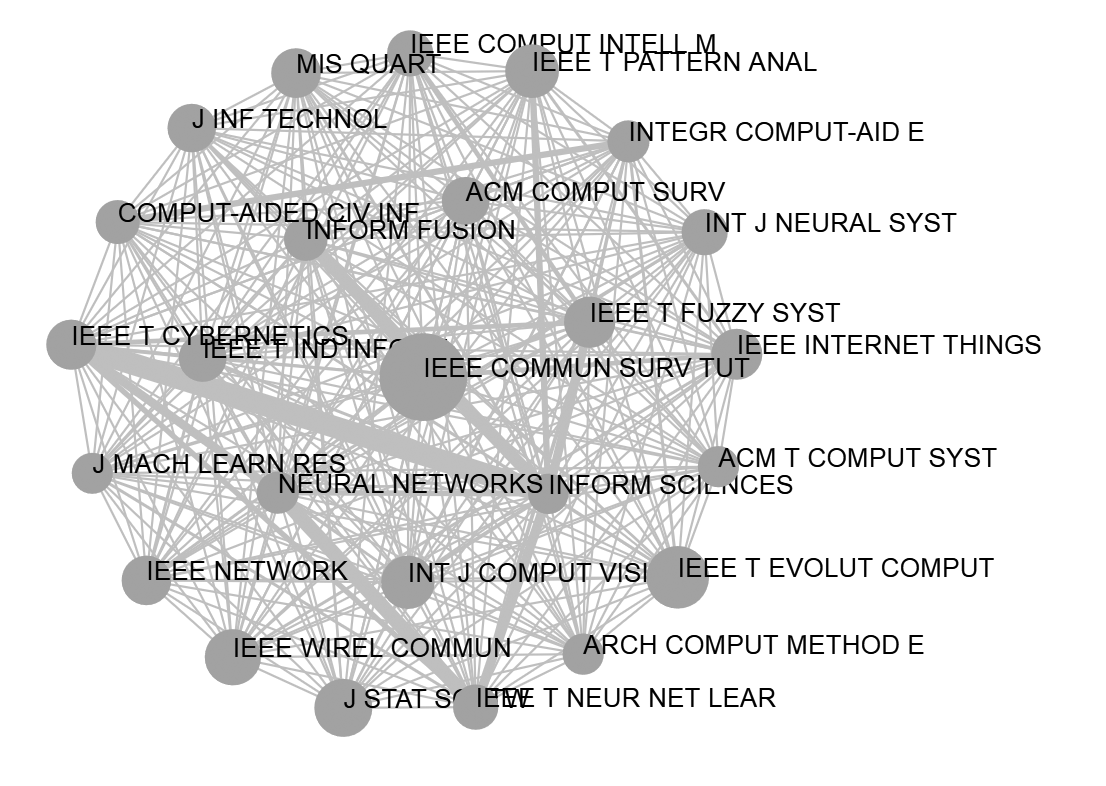
\includegraphics[width=2.5in]{cs_jif_graph}
	\caption{\textbf{Top 25 Computer Science Journals by Journal Impact Factor from InCites Journal Citation Report in 2016.} Gray circles represent the Journal Impact Factor, where higher Journal Impact Factor values are represented by larger sizes. Connected lines represent the citation relationships between each journal, where thicker lines mean stronger relationships.}
	\label{figure:cs_jif_graph}
\end{figure}


\subsection{Automatic Search Queries} \label{automatic-search-queries}

Potential papers were found using search queries passed to the search engines of the ACM and IEEE Xplore digital libraries identified in Section \ref{digital-library-selections} \cite{ACM:2017,IEEE:2017}. Search queries were modified from the defaults and sorted by relevance (See Appendix \ref{appendix:acm_querysyntax} and \ref{appendix:ieeexplore_commandsearch}). Each search query was defined to filter for potential papers with the following requirements:

\begin{enumerate}[label=(\alph*)]
	\item \textbf{Publication}: Published in ACM or IEEE
	\item \textbf{Year}: Published from 2014 to October 5, 2017
	\item \textbf{Keywords}: Contains the keywords \textit{"hyperparameter"} and \textit{"optimization"} in the paper title
\end{enumerate}


\subsection{Manual Selection Criteria} \label{manual-selection-criteria}

The potential papers resulting from the methods in Section \ref{automatic-search-queries} were further filtered by inspecting the abstracts and paper length. The abstracts were inspected for relevancy to the topic: \textit{"hyperparameter optimization for machine learning"}. This included mentions of methods that deal with optimizing parameters for machine learning models to improve performance. After inspections of the abstract, each paper was further evaluated for practicality by searching for mentions of applications, benchmarks, and experiments in the results sections. It was assumed that papers with lengths of more than 8 pages provided adequate details and explanations of methods and results. The manual selection criteria sought to find papers with the following characteristics:

\begin{enumerate}[label=(\alph*)]
	\item \textbf{Detailed}: Paper contained adequate details and explanations of methods and results with the assumption that papers with 8 or more pages satisfied this criteria
	\item \textbf{Relevant}: Paper had mentions of hyperparameter optimization methods for machine learning models
	\item \textbf{Practical}: Paper had conducted experiments, benchmarks, or applications of hyperparameter optimization methods
\end{enumerate}


\subsection{Review Procedure} \label{review-procedure}

A literature review of the papers selected using the methods in Section \ref{manual-selection-criteria} was done with the following procedure:

\begin{enumerate}
	\item \textbf{Identify} methods used for hyperparameter optimization of machine learning models
	\item \textbf{Summarize} methods in (1)
	\item \textbf{Summarize} experiments and results for the methods in (1)
	\item \textbf{Discuss} limitations, possible improvements, and future directions relative to the summaries from (2) and (3)
\end{enumerate}


% *** RESULTS ***


\section{Results} \label{results}

This section details the selected papers and review procedure results described in Section \ref{methods}. Papers were selected from 2015 to October 5, 2017 as described in Section \ref{selected-papers}, where a majority of the potential and selected papers were from the IEEE Xplore digital library. Summaries of the hyperparameter optimization methods, data, and experiments from the selected papers are provided in Sections \ref{hyperparameter-optimization-methods}, and \ref{data-and-experiments} respectively.


\subsection{Selected Papers} \label{selected-papers}

A total of five papers were selected for this review after applying the search queries described in Section \ref{automatic-search-queries} and selection criteria described in Section \ref{manual-selection-criteria}. The search queries resulted in 14 potential papers, where 2 were from the ACM digital library, and 12 were from the IEEE Xplore digital library as seen in Figure \ref{figure:papers_library}. The number of potential papers and selected papers for each year from 2014 to 2017 is seen in Figure \ref{figure:papers_yearly}. The five papers selected for this review are seen in Table \ref{table:papers_selected}, where a majority of papers were from the IEEE Xplore digital library.

\begin{table}
\centering
\caption{\textbf{Selected Papers for Literature Review.} Papers were selected according to search queries described in Section \ref{automatic-search-queries} and selection criteria described in Section \ref{manual-selection-criteria}. Papers are sorted in ascending order by year and then alphabetically by the first author's last name.}
\label{table:papers_selected}
\begin{tabular}{p{1in}p{1.25in}p{0.2in}p{0.3in}}
	\toprule
	\textbf{Authors} & \textbf{Title} & \textbf{Year} & \textbf{Library} \\
	\midrule \addlinespace
	Schilling N., Wistuba M., Drumond L., Schmidt-Thieme L. \cite{Schilling:2015} & Joint Model Choice and Hyperparameter Optimization with Factorized Multilayer Perceptrons & 2015 & IEEE
	\addlinespace\\ 
	\midrule \addlinespace
	Wistuba M., Schilling N., Schmidt-Thieme L. \cite{Wistuba:2015} & Learning Hyperparameter Optimization Initializations & 2015 & IEEE
	\addlinespace \\
	\midrule \addlinespace
	Wistuba M., Schilling N., Schmidt-Thieme L. \cite{Wistuba:2016} & Hyperparameter Optimization Machines & 2016 & IEEE 
	\addlinespace \\
	\midrule \addlinespace
	L\`evesque J-C., Durand A., Gagn\`e C., Sabourin R. \cite{Levesque:2017}& Bayesian Optimization for Conditional Hyperparameter Spaces & 2017 & IEEE
	\addlinespace \\ 
	\midrule \addlinespace
	Quitadamo A., Johnson J., Shi X. \cite{Quitadamo:2017}& Bayesian Hyperparameter Optimization for Machine Learning Based eQTL Analysis & 2017 & ACM 
	\addlinespace \\
	\bottomrule
\end{tabular}
\end{table}

\begin{figure}
\begin{center}
\begin{tikzpicture}
\begin{axis}[
	ylabel=Papers,
	xlabel=Year,
	ybar interval=1,
	xticklabel style={/pgf/number format/1000 sep=,},
	legend style={
	  at={(0.5,-0.20)},
	  anchor=north,
	  legend columns=-1
	}
	]
	\addplot[color=black, fill=gray] table[x=year, y=papers_acm] {data/papers_library.tsv};
	\addplot[color=black, fill=black] table[x=year, y=papers_ieee] {data/papers_library.tsv};
	\legend{\strut ACM, \strut IEEE Xplore}
\end{axis}
\end{tikzpicture}
\caption{\textbf{Potential ACM and IEEE Published Papers Found from 2014 to October 5, 2017.} Gray bars represent the potential papers found from the ACM digital library, and black bars represent the potential papers from IEEE Xplore digital library. Potential papers were found with search queries as described in Section \ref{automatic-search-queries}.}
\label{figure:papers_library}
\end{center}
\end{figure}

\begin{figure}
\begin{center}
\begin{tikzpicture}
\begin{axis}[
	ylabel=Papers,
	xlabel=Year,
	ybar interval=1,
	xticklabel style={/pgf/number format/1000 sep=,},
	legend style={
	  at={(0.5,-0.20)},
	  anchor=north,
	  legend columns=-1
	}
	]
	\addplot[color=black, fill=gray] table[x=year, y=papers_searchqueries] {data/papers_yearly.tsv};
	\addplot[color=black, fill=black] table[x=year, y=papers_selectioncriteria] {data/papers_yearly.tsv};
	\legend{\strut Potential Papers, \strut Selected Papers}
\end{axis}
\end{tikzpicture}
\caption{\textbf{ACM and IEEE Published Papers Found from 2014 to October 5, 2017.} Gray bars represent the potential papers found using the search queries described in Section \ref{automatic-search-queries}. Black bars represent the selected papers filtered from the potential papers using the selection criteria described in Section \ref{manual-selection-criteria}.}
\label{figure:papers_yearly}
\end{center}
\end{figure}


\subsection{Hyperparameter Optimization Methods} \label{hyperparameter-optimization-methods}

Hyperparameter optimization methods search a set of machine learning parameters to maximize a performance measure, where higher values represent better performance.

A hyperparameter optimization method seeks to find a set of parameters $x_1 \dots x_n$ that maximize the performance measure function $f$ (often time-consuming to evaluate) as seen in Equation \ref{equation:hyperparameter_optimization}:

\begin{equation}
\label{equation:hyperparameter_optimization}
	\{x_1 \dots x_n\} \textrm{ such that} \operatorname{arg\,max}_{x_1 \dots x_n} f(x_1 \dots x_n)
\end{equation}

The set of parameters $x_1 \dots x_n$ is then a search space of possible user inputs to a machine learning model. The idea is to create constraints (manually done by human intervention) on $x_1 \dots x_n$ by limiting the range of values, number of iterations, or allowed running time \cite{Bergstra:2011}. A hyperparameter optimization method can then be used to select the best $x_1 \dots x_n$ based on these constraints.

Simple hyperparameter optimization methods mentioned in the selected papers included manual search, grid search, and random search \cite{Bergstra:2012}. A manual search requires the user to use a trial and error process to find a selection of parameter values on a machine learning algorithm that results in generally adequate performance. The user is usually guided by expertise on the algorithm and dataset or through external knowledge such as previous experiments, literature, or other relevant experts. Grid search involves limiting the search space of parameter values to a predefined range of values to search in. The predefined range of values is based on the discretion of the user, which requires knowledge of appropriate ranges to use for the machine learning algorithm and dataset. Random search is similar to grid search, except that the predefined range of values are randomized according to a probability distribution. The randomization process enables larger ranges to be defined as not all values in the range will be used, which reduces the time required to optimize the machine learning hyperparameters. Simple hyperparameter optimization methods (summarized in Table \ref{table:simple_methods}) are easy to implement and their effectiveness are based on the user's expertise of the machine learning algorithms and datasets chosen.

\begin{table}
\centering
\caption{\textbf{Simple Hyperparameter Optimization Methods.}}
\label{table:simple_methods}
\begin{tabular}{p{1in}p{2in}}
	\toprule
	\textbf{Method} & \textbf{Description}\\
	\midrule \addlinespace
	Manual Search & Trial and error attempt to find optimal hyperparameters
	\addlinespace\\ 
	Grid Search & Predefined range of values to limit optimal hyperparameter search space
	\addlinespace\\ 
	Random Search & Randomized range of values to limit optimal hyperparameter search space
	\addlinespace \\
	\bottomrule
\end{tabular}
\end{table}

Advanced hyperparameter optimization methods in the selected papers included assumption based optimization, evolutionary based optimization, and Sequential Model Based Optimization (SMBO). Assumption based optimization creates particular hyperparameter models for particular algorithms, datasets, and situations \cite{Schilling:2015}. Evolutionary based optimization uses evolutionary algorithms, inspired by biology, to search for optimal hyperparameters in machine learning models \cite{Whitley:1996}. These evolutionary algorithms produce several machine learning models varied by hyperparameter values, evolves these produced models by mutation, and selects the best performing evolved models. SMBO creates a model of the performance measure function, treated as a black-box function, to predict the next best set of hyperparameters to evaluate \cite{Jones:1998}. Gaussian models (Bayesian optimization) \cite{Snoek:2012} and random forest models \cite{Hutter:2011} have been used in SMBO to model the performance measure function in order to find optimal hyperparameters. Advanced hyperparameter optimization methods (summarized in Table \ref{table:advanced_methods}) provide more efficient and effective approaches than simple hyperparameter optimization methods under the same constraints such as number of iterations or allowed running time.

\begin{table}
\centering
\caption{\textbf{Advanced Hyperparameter Optimization Methods.}}
\label{table:advanced_methods}
\begin{tabular}{p{1.25in}p{2in}}
	\toprule
	\textbf{Method} & \textbf{Description}\\
	\midrule \addlinespace
	Assumption Based & Specific hyperparameter models based on expert assumptions of particular algorithms and datasets
	\addlinespace\\ 
	Evolutionary Based & Models that attempt to select the best performing hyperparameters from a set of procedurally generated hyperparameters
	\addlinespace\\ 
	Sequential Model Based & Models of the performance measure function to sequentially guide the next hyperparameters to be evaluated
	\addlinespace \\
	\bottomrule
\end{tabular}
\end{table}

Several improvements to SMBO have been proposed by the authors of the selected papers. Schilling, Wistuba, Drumond, and Schmidt-Thieme \cite{Schilling:2015} used factorized multilayer perceptions to form lower dimensional spaces. The integration of the factorized multilayer perceptron model into the SMBO allowed SMBO to search for optimal hyperparameters across different datasets and machine learning algorithms. Wistuba, Schilling, and Schmidt-Thieme \cite{Wistuba:2015} used an initialization learning algorithm to transfer more optimal initial hyperparameter values from previous experiments. This enabled more efficient searching by providing more optimal starting values for the search space in hyperparameter optimization methods. Wistuba, Schilling, and Schmidt-Thieme \cite{Wistuba:2016} proposed an improved framework over SMBO called Hyperparameter Optimization Machines (HOM) that used a transfer function in addition to the original model in SMBO. The transfer function controlled the influence of transferred hyperparameter knowledge from previous experiments such that hyperparameter values can become irrelevant once enough data about the search space is gathered. L\`evesque, Durand, Gagn\`e, and Sabourin \cite{Levesque:2017} proposed conditional kernels for Bayesian optimization (a SMBO method) that handled conditional hyperparameter spaces with Gaussian Processes. Conditional hyperparameter spaces occurred when there were hyperparameters that were dependent on other hyperparameters or had the ability to be inactive (having no value). A summary of the improvements to SMBO are provided in Table \ref{table:smbo_improvements}.

\begin{table}
\centering
\caption{\textbf{Sequential Model Based Optimization Improvements.}}
\label{table:smbo_improvements}
\begin{tabular}{p{1in}p{0.7in}p{1.3in}}
	\toprule
	\textbf{Authors} & \textbf{Method} & \textbf{Improvement} \\
	\midrule \addlinespace
	Schilling N., Wistuba M., Drumond L., Schmidt-Thieme L. \cite{Schilling:2015} & Factorized multilayer perceptron & Enabled hyperparameter optimization across different datasets and machine learning algorithms
	\addlinespace\\ 
	\midrule \addlinespace
	Wistuba M., Schilling N., Schmidt-Thieme L. \cite{Wistuba:2015} & Hyperparameter initialization learning & Provided more optimal starting points in hyperparameter search space
	\addlinespace \\
	\midrule \addlinespace
	Wistuba M., Schilling N., Schmidt-Thieme L. \cite{Wistuba:2016} & Hyperparameter Optimization Machines (HOM)  & Provided a way to measure the influence of transferred hyperparameter values from previous experiments
	\addlinespace \\
	\midrule \addlinespace
	L\`evesque J-C., Durand A., Gagn\`e C., Sabourin R. \cite{Levesque:2017}& Conditional kernels & Provided a method to optimize for hyperparameters that are dependent on other hyperparameters or have the ability to be inactive
	\addlinespace \\
	\bottomrule
\end{tabular}
\end{table}


\subsection{Data and Experiments} \label{data-and-experiments}

The selected papers ran experiments on the several hyperparameter optimization methods to evaluate and compare their performance:

\subsubsection{Schilling, Wistuba, Drumond, and Schmidt-Thieme (2015)}

Schilling et al. \cite{Schilling:2015} performed experiments\footnote{The experiments and data overview are publicly available at: http://www.hylap.org} for 59 created datasets\footnote{The 59 created datasets were from the Waikato Environment for Knowledge Analysis (WEKA) \cite{Hall:2009} machine learning software.} with 1873 subsample hyperparameter configurations for 4 hyperparameter optimization methods. The results revealed that factored multilayer perceptrons models achieved greater normalized accuracy (90\% versus 70\%) for the same machine learning algorithms at earlier points in time by learning initializations from meta-data\footnote{Meta-data contain data that are directly or indirectly related to other data. This meta-data provides simplified information (such as titles, dates, and locations) and possibly hidden structural patterns on other data that can improve the performance of hyperparameter optimization algorithms.} sets.

\subsubsection{Wistuba, Schilling, and Schmidt-Thieme (2015)}

Wistuba et al. \cite{Wistuba:2015} performed experiments that compared hyperparameter optimization methods with and without initialized hyperparameter values based on 80\% training and 20\% testing splits of 50 classification datasets\footnote{The datasets were generated from A Library for Support Vector Machines (LIBSVM) \cite{Chang:2011} and MultiBoost \cite{Benbouzid:2012} machine learning libraries.}. The results revealed that the hyperparameter optimization methods with initialized hyperparameter values performed better due to initialization learning from previous experiments.

\subsubsection{Wistuba, Schilling, and Schmidt-Thieme (2016)}

Wistuba et al. \cite{Wistuba:2016} later performed experiments on two different meta-data sets\footnote{The two datasets were generated by the machine learning libraries A Library for LIBSVM \cite{Chang:2011} and WEKA \cite{Hall:2009} with 50 datasets and 59 datasets respectively.} for hyperparameter optimization and combined algorithm selection. The results revealed that a HOM framework with Adaptive Hyperparameter Transfer Learning with Simple Surrogates (AHT) provided the best results in terms of space and time compared to regular initialization with SMBO.

\subsubsection{L\`evesque, Durand, Gagn\`e, and Sabourin (2017)}

L\`evesque et al. \cite{Levesque:2017} performed experiments on hyperparameter optimization methods with and without conditional kernels on 24 datasets\footnote{The 24 datasets were extracted from the OpenML repository \cite{Vanschoren:2014} and University of California Irvine (UCI) machine learning repository \cite{Lichman:2013}.} that consisted of 500 to 60000 instances. The results revealed that the hyperparameter optimization methods with conditional kernels outperformed other optimization methods that did not use conditional kernels on the datasets.

\subsubsection{Quitadamo, Johnson, and Shi (2017)}

Quitadamo, Johnson, and Shi \cite{Quitadamo:2017} performed experiments of hyperparameter optimization on large genomic datasets\footnote{The datasets were extracted from the 1000 Genomes project \cite{Sudmant:2015} and Genetic European Variation in Health and Disease (gEUVADIS) project \cite{Lappalainen:2013}.}, where the number of columns are significantly larger than the number of rows, for the methods of grid search, random search, and Bayesian optimization. The results revealed that Bayesian optimization found better parameters than grid search or random search in  the same amount of time for the genomic dataset.

The datasets used for the mentioned experiments used publicly available datasets generated from popular machine learning libraries and repositories as seen in Table \ref{table:datasets} (with the exception of Quitadamo et al. \cite{Quitadamo:2017}). The hyperparameter optimization methods that had high performance incorporated the SMBO framework with initialization of hyperparameter values from transfer learning techniques.

\begin{table}
\centering
\caption{\textbf{Datasets Used in Selected Papers.}}
\label{table:datasets}
\begin{tabular}{p{2.25in}p{0.75in}}
	\toprule
	\textbf{Dataset} & \textbf{\# Papers} \\
	\midrule \addlinespace
	1000 Genomes project \cite{Sudmant:2015} & 1 \cite{Quitadamo:2017}
	\addlinespace\\ 
	\midrule \addlinespace
	A Library for Support Vector Machines (LIBSVM) \cite{Chang:2011} & 2 \cite{Wistuba:2015} \cite{Wistuba:2016}
	\addlinespace\\ 
	\midrule \addlinespace
	Genetic European Variation in Health and Disease (gEUVADIS) project \cite{Lappalainen:2013} & 1 \cite{Quitadamo:2017}
	\addlinespace\\ 
	\midrule \addlinespace
	MultiBoost \cite{Benbouzid:2012} & 1 \cite{Wistuba:2015}
	\addlinespace \\
	\midrule \addlinespace
	OpenML \cite{Vanschoren:2014} & 1 \cite{Levesque:2017}
	\addlinespace \\
	\midrule \addlinespace
	University of California Irvine (UCI) Machine Learning Repository \cite{Lichman:2013} & 1 \cite{Levesque:2017}
	\addlinespace \\
	\midrule \addlinespace
	Waikato Environment for Knowledge Analysis (WEKA) \cite{Hall:2009} & 2 \cite{Schilling:2015} \cite{Wistuba:2016}
	\addlinespace \\
	\bottomrule
\end{tabular}
\end{table}


% *** DISCUSSION ***


\section{Discussion} \label{discussion}

This section discusses the limitations, proposed improvements, and future directions for the selected papers in Table \ref{table:papers_selected}. Section \ref{limitations} discusses the limitations of hyperparameter optimization relative to dimensionality, dataset characteristics, and machine learning algorithm choice. Section \ref{improvements-and-future-directions} discusses the proposed improvements and future research directions relative to sampling, model combination, and automated machine learning.


\subsection{Limitations} \label{limitations}

The limitations of hyperparameter optimization methods for machine learning algorithms include issues with high dimensional hyperparameters, large datasets, costly performance measure functions, and variations between datasets. High dimensional hyperparameters lead to longer evaluation times for the performance measure function, which may noticeably  lower the plausible search space. Extremely large datasets, similar to high dimensional hyperparameters, also increase the evaluation times for the performance measure function, which reduces may drastically reduce the plausible search space. The running time constraint is also heavily influenced by the time expense of the performance measure functions. If the performance measure functions are not scalable, hyperparameter optimization methods can not gather enough data in feasible times to produce an adequate model. Hyperparameter optimization methods also vary between different datasets, and there does not exist one method that will provide the best results in every scenario. Although hyperparameter optimization methods are effective for producing machine learning models with high performance, the methods are not entirely automatic (human intervention is required to select the parameter ranges, and time constraints) and are heavily reliant on the machine learning algorithms and the datasets being used.


\subsection{Improvements and Future Directions} \label{improvements-and-future-directions}

The improvements and future directions of hyperparameter optimization methods for learning algorithms include sampling techniques, combination of machine learning models, and automated machine learning. Results from hyperparameter optimization are highly dependent on the datasets and machine learning algorithms used. The dimensionality of the dataset and hyperparameters can affect the plausibility of running optimization methods. Sampling techniques can help reduce the dimensionality and the size of datasets and hyperparameters in order to improve running times, and time constraints on hyperparameter optimization methods. The combination of machine learning models and algorithms should be considered to produce new machine learning models that have the potential to out perform the models if they were not combined. Combining machine learning models through hyperparameter optimization methods may lead into the direction of automated machine learning, where new models can be created and adjusted without human intervention.


% *** CONCLUSION ***


\section{Conclusion} \label{conclusion}

This review selected papers from the ACM and IEEE Xplore digital libraries by evaluating journal citation reports, using automatic search queries, and applying manual selection criteria. The review methods limited the papers to content relevant to hyperparameter optimization methods for machine learning for the years 2015 to 2017. The five selected papers were summarized for optimization methods, improvements, and experiments for an overview of the recent advances in hyperparameter optimization. Sequential Model Based Optimization (SMBO) was a common framework used among all papers, where comparisons and improvements were made to SMBO. Improvements to hyperparameter optimization methods included the use of hyperparameter initialization techniques and the inclusion of conditional hyperparameter spaces. However, hyperparameter optimization methods are highly reliant on the datasets and machine learning algorithms used, which may pose issues in requiring human intervention, inconsistent results, and time constraints. Sampling was proposed as a possible solution to combat the limitations of high dimensionality in the datasets and hyperparameters. The application of hyperparameter optimization to the process of combining machine learning models was also proposed as a way to automatically create new machine learning models. Work towards improving and applying hyperparameter optimization methods may lead to advances in automated machine learning.

